\section{Model Equations}
\Figref{diagramQuad} shows a representation of the quadcopter where two reference systems, inertial and body, can be seen, as well as the conventions for angles of rotation and forces. \Figref{diagramTorque} shows the body from above and includes the chosen convention for the torques produced by the propellers.
 
\begin{minipage}{\linewidth}
	\begin{minipage}{0.45\linewidth}
		\begin{figure}[H]
			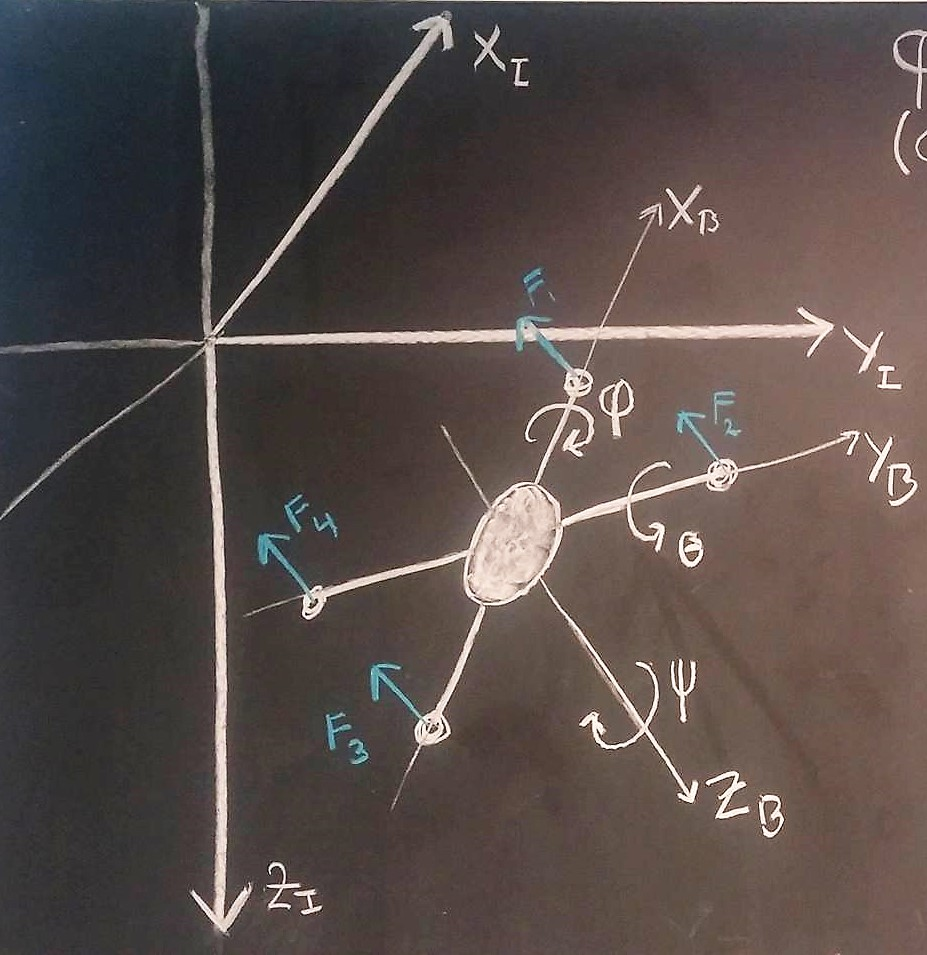
\includegraphics[scale=.27]{figures/drone_diagram}
			\centering
			\captionsetup{justification=centering}
			\captionof{figure}{Diagram of the quadcopter which includes inertial and body reference systems, as well as the references for the angles (roll, pitch and yaw) and the thrust forces produced by the propeller. }
			\label{diagramQuad}
		\end{figure}
	\end{minipage}
	\hspace{0.03\linewidth}
	\begin{minipage}{0.45\linewidth}
		\begin{figure}[H] \vspace{16mm}
			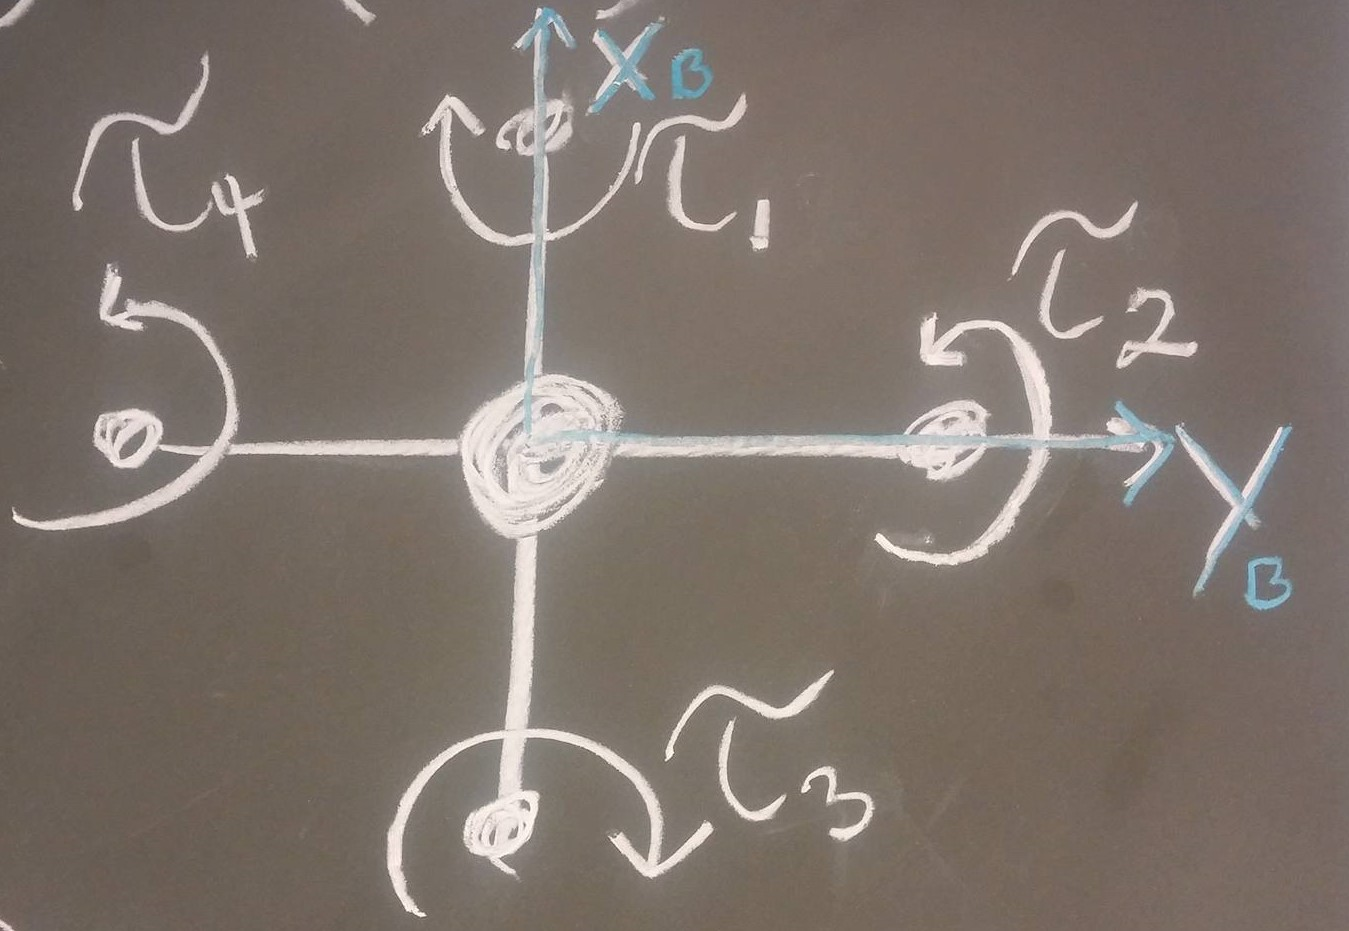
\includegraphics[scale=.18]{figures/torques_diagram}
			\centering
			\captionsetup{justification=centering}
			\captionof{figure}{Diagram of the quadcopter from above, with the references for the torques produced by the drag force at the propeller.}
			\label{diagramTorque}
		\end{figure}
	\end{minipage}
\end{minipage}
%
%\si{\phi} roll (around x-axis)\\ \\ 
%\si{\theta} pitch (around y-axis)\\ \\
%\si{\psi} yaw (around z-axis)\\
%
\subsection{Angular Accelerations}
From the diagrams above, the equations of angular motion along the three body axes can be derived.
%
\begin{flalign}
\eq{ J_x\cdot\ddot{\phi} }{(F_4-F_2)\cdot L} &\\
\eq{J_y \cdot\ddot{\theta}}{(F_1-F_3)\cdot L} &\\
\eq{J_z\cdot\ddot{\psi}}{\tau_1-\tau_2+\tau_3-\tau_4}
\label{eq:AngleEq}
\end{flalign}
%
\hspace{6mm} Where:\\
\begin{tabular}{ p{1cm} l l l}
	& \si{\ddot{\phi}} 	 	& is roll angular acceleration   	&\unitWh{rad \cdot s^{-2}} \\
	& \si{\ddot{\theta}} 	& is  pitch angular acceleration   &\unitWh{rad \cdot s^{-2}} \\
	& \si{\ddot{\psi}}	    & is yaw angular acceleration      &\unitWh{rad \cdot s^{-2}} \\
	& \si{J_x}  			& is the body moment of inertia around \si{x_B} direction       &\unitWh{kg \cdot m^2} \\
	& \si{J_y}          	& is the body moment of inertia around \si{y_B} direction        &\unitWh{kg \cdot m^2} \\
	& \si{J_z}          	& is the body moment of inertia around \si{z_B} direction        &\unitWh{kg \cdot m^2} \\	
	& \si{L}  				& is the length of the arm of the quadcopter      &\unitWh{m} \\
	& \si{F_n}          	& is the thrust force produced in each propeller        &\unitWh{N} \\
	& \si{\tau_n}          	& is the torque due to the drag force in each propeller        &\unitWh{N \cdot m} \\		
\end{tabular}

As it can be seen in the \eqref{eq:AngleEq}, the roll and pitch angular accelerations depend on the thrust forces exerted by the propellers placed in the y and x axes of the quadcopter, respectively. The yaw angle changes only due to the torques created by the drag force in the propeller.

The thrust forces and drag torques from the propeller can be approximated by terms depending on the velocity of the motor, which are found as described in Appendix \ref{}. The equations above can be rewritten to include these terms.
%
\begin{flalign}
	\eq{ J_x\cdot\ddot{\phi} }{k_{th} \cdot(\omega^2_4-\omega^2_2) \cdot L} &\\
	\eq{J_y \cdot\ddot{\theta}}{k_{th} \cdot(\omega^2_1-\omega^2_3) \cdot L} &\\
	\eq{J_z\cdot\ddot{\psi}}{k_d \cdot(\omega^2_1-\omega^2_2+\omega^2_3-\omega^2_4)}
	\label{eq:AngleEqVelocities}
\end{flalign}
%
\hspace{6mm} Where:\\
\begin{tabular}{ p{1cm} l l l}	
	& \si{k_{th}}  			& is the thrust constant      					&\unitWh{N \cdot s^2 \cdot m^{-2}} \\
	& \si{k_d}          	& is the drag constant        					&\unitWh{N \cdot m \cdot s^2 \cdot m^{-2}} \\
	& \si{\omega_n}         & is the angular velocity of the nth motor      &\unitWh{rad \cdot s^{-1}}	
\end{tabular}

\subsection{Linear Accelerations - Body Frame}
The linear acceleration components along the body coordinate frame directions evolve according to the equations below. They come from applying Newton's second law. As the gravity needs to be transformed from the inertial frame to the body frame, it has been multiplied by the rotation matrix (\eqref{rotMatrix}) that depends on the roll, pitch and yaw angles.
%
\begin{flalign}
	\eq{m\cdot\ddot{x}_B}{F_g(-\cos(\phi) \sin(\theta) \cos(\psi) + \sin(\phi) \sin (\psi))} &\\
	\eq{m\cdot\ddot{y}_B}{F_g(\cos(\phi) \sin(\theta) \sin(\psi) + \sin(\phi) \cos(\psi))}&\\
	\eq{m\cdot\ddot{z}_B}{-(F_1+F_2+F_3+F_4)+F_g\cdot \cos(\phi)\cos(\theta)}
\label{eq:AccelerationEqBody}
\end{flalign}
%
\hspace{6mm} Where:\\
\begin{tabular}{ p{1cm} l l l}
	& \si{\ddot{x_B}} 	 	& is the linear acceleration in \si{x_B} direction 	&\unitWh{m \cdot s^{-2}} \\
	& \si{\ddot{y_B}} 		& is the linear acceleration in \si{y_B} direction   &\unitWh{m \cdot s^{-2}} \\
	& \si{\ddot{z_B}}	    & is the linear acceleration in \si{x_B} direction     &\unitWh{m \cdot s^{-2}} \\
	& \si{\phi}	 			& is the roll position 	&\unitWh{rad} \\
	& \si{\theta} 			& is the pitch position    &\unitWh{rad} \\
	& \si{\psi}    			& is the yaw position      &\unitWh{rad} \\
	& \si{F_g}    			& is the magnitude of the gravity force      &\unitWh{N} \\
\end{tabular}


As happened with the equations of the angular movement, the forces and torques can be written as a function of the motors' speeds.
\begin{flalign}
	\eq{m\cdot\ddot{x}_B}{F_g(-\cos(\phi) \sin(\theta) \cos(\psi) + \sin(\phi) \sin (\psi))} &\\
	\eq{m\cdot\ddot{y}_B}{F_g(\cos(\phi) \sin(\theta) \sin(\psi) + \sin(\phi) \cos(\psi))}&\\
	\eq{m\cdot\ddot{z}_B}{-k_{th}\cdot(\omega^2_1+\omega^2_2+\omega^2_3+\omega^2_4)+F_g\cdot \cos(\phi)\cos(\theta)}
	\label{eq:AccelerationEqBodyVelocities}
\end{flalign}

The transformation of the gravity force is explained by three consecutive rotations (roll, pitch and yaw) combined in one rotation matrix \si{R_{\phi, \theta, \psi}}.

\begin{minipage}{0.3\linewidth}
	\begin{flalign}
		\si{R_\phi} &=
		\begin{bmatrix}
			\ \si{1}                & \si{0}                & \si{0} \ \ \ \\ 
			\ \si{0}  				& \si{c(\phi)} 		& \si{-s(\phi)}                 \ \ \ \\ 
			\ \si{0}                & \si{s(\phi)}       & \si{c(\phi)}                  \ \ \  
		\end{bmatrix}  \nonumber 
	\end{flalign}
\end{minipage}\hfill
%
\begin{minipage}{0.3\linewidth}
	\begin{flalign}
		\si{R_\theta} &=
		\begin{bmatrix}
			\ \si{c(\theta)}      & \si{0}       & \si{s(\theta)} \ \ \ \\ 
			\ \si{0}  				& \si{1} 	   & \si{0}                 \ \ \ \\ 
			\ \si{-s(\theta)}     & \si{0}       & \si{c(\theta)}                  \ \ \  
		\end{bmatrix}   \nonumber 
	\end{flalign}
\end{minipage}\hfill
%
\begin{minipage}{0.3\linewidth}
	\begin{flalign}
		\si{R_\phi} &=
		\begin{bmatrix}
			\ \si{c(\psi)}                & \si{-s(\psi)}                & \si{0} \ \ \ \\ 
			\ \si{s(\psi)}  				& \si{c(\psi)} 		& \si{0}                 \ \ \ \\ 
			\ \si{0}                & \si{0}       & \si{1}                  \ \ \  
		\end{bmatrix} \nonumber 
	\end{flalign}
\end{minipage}\hfill

\begin{flalign}
	\si{R_{\phi, \theta, \psi}} &=
	\begin{bmatrix}
		\ \si{c(\theta) \cdot c(\psi)}                & \si{-c(\theta) \cdot s(\psi)}  & \si{s(\theta)} \ \ \ \\ 
		\ \si{s(\phi) \cdot s(\theta) \cdot s(\psi) + c(\phi) \cdot s(\psi)}  	  & \si{-s(\phi) \cdot s(\theta) \cdot s(\psi) + c(\phi) \cdot c(\psi)} 		& \si{-s(\phi) \cdot c(\theta)}                 \ \ \ \\ 
		\ \si{-c(\phi) \cdot s(\theta) \cdot c(\psi) + s(\phi) \cdot s(\psi)}  	  & \si{c(\phi) \cdot s(\theta) \cdot s(\psi) + s(\phi) \cdot c(\psi)} 		& \si{c(\phi) \cdot c(\theta)}                 \ \ \ 
	\end{bmatrix} 	\label{rotMatrix}
\end{flalign}


\subsection{Linear Accelerations - Inertial Frame}
It is also possible to explain the linear acceleration in the inertial reference frame. This approach is useful if the aim of the controller is to give references of acceleration, velocity or position in this frame.

In this case the gravity force has effect only in the \si{z_B} direction and the four forces from the motors need to be transformed into the inertial system. This is done using the inverse of the rotation matrix (\eqref{invRotMatrix}).
%
\begin{flalign}
	\eq{m\cdot\ddot{x}_I}{-(F1+F2+F3+F4)\cdot\sin(\theta)} &\\
	\eq{m\cdot\ddot{y}_I}{-(F1+F2+F3+F4)\cdot(-\sin(\phi))\cdot\cos(\theta)} &\\
	\eq{m\cdot\ddot{z}_I}{F_g-(F1+F2+F3+F4)\cdot\cos(\phi)\cdot\cos(\theta)}
	\label{eq:AccelerationEqInertial}
\end{flalign}
%
\hspace{6mm} Where:\\
\begin{tabular}{ p{1cm} l l l}
	& \si{\ddot{x_I}} 	 	& is the linear acceleration in \si{x_I} direction 	&\unitWh{m \cdot s^{-2}} \\
	& \si{\ddot{y_I}} 		& is the linear acceleration in \si{y_I} direction   &\unitWh{m \cdot s^{-2}} \\
	& \si{\ddot{z_I}}	    & is the linear acceleration in \si{x_I} direction     &\unitWh{m \cdot s^{-2}} \\
\end{tabular}


\begin{flalign}
	\eq{m\cdot\ddot{x}_I}{-k_{th}\cdot({\omega_1}^2+{\omega_2}^2+{\omega_3}^2+{\omega_4}^2)\cdot\sin(\theta)} &\\
	\eq{m\cdot\ddot{y}_I}{-k_{th}\cdot({\omega_1}^2+{\omega_2}^2+{\omega_3}^2+{\omega_4}^2)\cdot(-\sin(\phi))\cdot\cos(\theta)} &\\
	\eq{m\cdot\ddot{z}_I}{F_g-k_{th}\cdot({\omega_1}^2+{\omega_2}^2+{\omega_3}^2+{\omega_4}^2)\cdot\cos(\phi)\cdot\cos(\theta)}
	\label{eq:AccelerationEqInertialVelocities}
\end{flalign}
%
\small
\begin{flalign}
	\si{R^{-1}_{\phi, \theta, \psi}} &=
	\begin{bmatrix}
		\ \si{c(\theta) \cdot c(\psi)}                & \si{-c(\theta) \cdot s(\psi)}  & \si{-c(\phi) \cdot s(\theta) \cdot c(\psi) + s(\phi) \cdot s(\psi)}  \ \ \ \\ 
		\ \si{s(\phi) \cdot s(\theta) \cdot s(\psi) + c(\phi) \cdot s(\psi)}  	  & \si{-s(\phi) \cdot s(\theta) \cdot s(\psi) + c(\phi) \cdot c(\psi)} 		& \si{c(\phi) \cdot s(\theta) \cdot s(\psi) + s(\phi) \cdot c(\psi)}                \ \ \ \\ 
		\ \si{s(\theta)}      	  & \si{-s(\phi) \cdot c(\theta)}    		& \si{c(\phi) \cdot c(\theta)}                 \ \ \ 
	\end{bmatrix} 	\label{invRotMatrix}
\end{flalign}
\normalsize

\section{Linearization of the Equations}
Since the goal is to design a linear controller it is necessary to linearize the equations that contains around the equilibrium point. This is done using the first order Taylor approximation in each equation.
\begin{flalign}
	\eq{J_x\cdot\Delta\ddot{\phi}}{k_{th} \cdot L \cdot({\overline{\omega}^2_4}\cdot \Delta \omega_2-{\overline{\omega}^2_2}\cdot \Delta \omega_4)}&\\
	\eq{J_x\cdot\Delta\ddot{\theta}}{k_{th} \cdot L \cdot({\overline{\omega}^2_1}\cdot \Delta \omega_1-{\overline{\omega}^2_3}\cdot \Delta \omega_3)}&\\
	\eq{J_x\cdot\Delta\ddot{\psi}}{k_d \cdot ({\overline{\omega}^2_1}\cdot \Delta \omega_1+{\overline{\omega}^2_2}\cdot \Delta \omega_2+{\overline{\omega}^2_3}\cdot \Delta \omega_3+{\overline{\omega}^2_4}\cdot \Delta \omega_4)}&
\end{flalign}
%
\hspace{6mm} Where:\\
\begin{tabular}{ p{1cm} l l l}
	& \si{\Delta\ddot{\phi}} 	 	& is the change in roll angular acceleration from equilibrium  	&\unitWh{rad \cdot s^{-2}} \\
	& \si{\Delta\ddot{\theta}} 		& is the change in pitch angular acceleration from equilibrium   &\unitWh{rad \cdot s^{-2}} \\
	& \si{\Delta\ddot{\psi}}	    & is the change in yaw angular acceleration from equilibrium     &\unitWh{rad \cdot s^{-2}} \\
	& \si{\overline{\omega}^2_n}  	& is the angular velocity of the nth motor in equilibrium       &\unitWh{rad \cdot s^{-1}} \\
	& \si{\Delta \omega_n}          & is the change in angular velocity from equilibrium of the nth motor        &\unitWh{rad \cdot s^{-1}} \\
\end{tabular}

\begin{flalign}
	\eqOne{m\cdot\Delta\ddot{x}_I}{(-k_{th}\cdot(2\textbf{ }{\overline{\omega}_1}^2\cdot\Delta\omega_1+2\textbf{ }{\overline{\omega}_2}^2\cdot\Delta\omega_2+2\textbf{ }{\overline{\omega}_3}^2\cdot\Delta\omega_3+2\textbf{ }{\overline{\omega}_4}^2\cdot\Delta\omega_4)\cdot\sin(\overline{\theta})-}
	\eqTwo{-k_{th}\cdot({\overline{\omega}_1}^2+{\overline{\omega}_2}^2+{\overline{\omega}_3}^2+{\overline{\omega}_4}^2)\cdot\cos(\overline{\theta})\Delta\theta} &\\
	\eqOne{m\cdot\Delta\ddot{y}_I}{(k_{th}\cdot(2\textbf{ }{\overline{\omega}_1}^2\cdot\Delta\omega_1+2\textbf{ }{\overline{\omega}_2}^2\cdot\Delta\omega_2+2\textbf{ }{\overline{\omega}_3}^2\cdot\Delta\omega_3+2\textbf{ }{\overline{\omega}_4}^2\cdot\Delta\omega_4)\cdot\sin(\overline{\phi})\cdot\cos(\overline{\theta})-}
	\eqTwo{-k_{th}\cdot({\overline{\omega}_1}^2+{\overline{\omega}_2}^2+{\overline{\omega}_3}^2+{\overline{\omega}_4}^2)\cdot\sin(\overline{\phi})\cdot\sin(\overline{\theta})\cdot\Delta\theta+}\nonumber\\
	\eqThree{+k_{th}\cdot({\overline{\omega}_1}^2+{\overline{\omega}_2}^2+{\overline{\omega}_3}^2+{\overline{\omega}_4}^2)\cdot\cos(\overline{\phi})\cdot\cos(\overline{\theta})\cdot\Delta\phi} &\\
	\eqOne{m\cdot\Delta\ddot{z}_I}{(-k_{th}\cdot(2\textbf{ }{\overline{\omega}_1}^2\cdot\Delta\omega_1+2\textbf{ }{\overline{\omega}_2}^2\cdot\Delta\omega_2+2\textbf{ }{\overline{\omega}_3}^2\cdot\Delta\omega_3+2\textbf{ }{\overline{\omega}_4}^2\cdot\Delta\omega_4)\cdot\cos(\overline{\phi})\cdot\cos(\overline{\theta})-}
	\eqTwo{-k_{th}\cdot({\overline{\omega}_1}^2+{\overline{\omega}_2}^2+{\overline{\omega}_3}^2+{\overline{\omega}_4}^2)\cdot\sin(\overline{\phi})\cdot\cos(\overline{\theta})\cdot\Delta\theta-}\nonumber\\
	\eqThree{-k_{th}\cdot({\overline{\omega}_1}^2+{\overline{\omega}_2}^2+{\overline{\omega}_3}^2+{\overline{\omega}_4}^2)\cdot\cos(\overline{\phi})\cdot\sin(\overline{\theta})\cdot\Delta\phi}
	\label{eq:LinearEquations}
\end{flalign}
%
\begin{flalign}
	\eq{m\cdot\Delta\ddot{x}_I}{-k_{th}\cdot({\overline{\omega}_1}^2+{\overline{\omega}_2}^2+{\overline{\omega}_3}^2+{\overline{\omega}_4}^2)\cdot\cos(\overline{\theta})\Delta\theta} &\\
	\eq{m\cdot\Delta\ddot{y}_I}{k_{th}\cdot({\overline{\omega}_1}^2+{\overline{\omega}_2}^2+{\overline{\omega}_3}^2+{\overline{\omega}_4}^2)\cdot\cos(\overline{\phi})\cdot\cos(\overline{\theta})\cdot\Delta\phi} &\\
	\eq{m\cdot\Delta\ddot{z}_I}{(-2\textbf{ }k_{th}\cdot({\overline{\omega}_1}^2\cdot\Delta\omega_1+{\overline{\omega}_2}^2\cdot\Delta\omega_2+{\overline{\omega}_3}^2\cdot\Delta\omega_3+{\overline{\omega}_4}^2\cdot\Delta\omega_4)\cdot\cos(\overline{\phi})\cdot\cos(\overline{\theta})}
	\label{eq:FinalLinearEquations}
\end{flalign}
%
\hspace{6mm} Where:\\
\begin{tabular}{ p{1cm} l l l}
	& \si{\Delta\ddot{x_I}} 	 	& is the change in linear acceleration from equilibrium in \si{x_I} direction 	&\unitWh{m \cdot s^{-2}} \\
	& \si{\Delta\ddot{y_I}} 		& is the change in linear acceleration from equilibrium in \si{y_I} direction   &\unitWh{m \cdot s^{-2}} \\
	& \si{\Delta\ddot{z_I}}	    	& is the change in linear acceleration from equilibrium in \si{z_I} direction     &\unitWh{m \cdot s^{-2}} \\
	& \si{\Delta \phi}	 			& is the change in roll position from equilibrium  	&\unitWh{rad} \\
	& \si{\Delta \theta} 			& is the change in pitch position from equilibrium   &\unitWh{rad} \\
	& \si{\Delta \psi}    			& is the change in yaw position from equilibrium     &\unitWh{rad} \\
	& \si{\overline{\phi}}	 			& is the roll position in equilibrium  	&\unitWh{rad} \\
	& \si{\overline{\theta}} 			& is the pitch position in equilibrium   &\unitWh{rad} \\
	& \si{\overline{\psi}}    			& is the yaw position in equilibrium     &\unitWh{rad} \\
\end{tabular}





